


%%%%%%%%%%%%%%%%%%%%%%%%%%%%%%%%%%%%%%%%%%%%%%%%%%%%%%%%%%%%%%%%%%%%%%%%
%%%%%% Definitionen
%%%%%%%%%%%%%%%%%%%%%%%%%%%%%%%%%%%%%%%%%%%%%%%%%%%%%%%%%%%%%%%%%%%%%%%%

\section{Mathematische Definitionen}
Zu Beginn definieren wir die grundlegenden mathematischen Begriffe. Als wichtigste Grundlage dient 
hierbei das Konstrukt des \red{ungerichteten} Graphen.
\begin{definition}[Graph] ~\\
Ein (ungerichteter) \textbf{Graph} $G = (V,E)$ ist ein Tupel bestehend aus einer Knotenmenge $V$ und einer Kantenmenge
 $E$. Eine Kante verbindet zwei Knoten miteinander und ist damit eine Menge, aus zwei Knoten.
 Es gilt: $E \subseteq \{ \{u,v\} |\ u,v \in V, u \neq v \}$.  
\end{definition}
\red{In dieser Arbeit} spielt eine spezielle Klasse von Graphen, bipartite Graphen, eine zentrale Rolle.
Bei einem bipartiten Graphen kann man die Knoten in zwei Mengen teilen, sodass alle Kanten nur zwischen den 
beiden Mengen verlaufen und nicht innerhalb einer Menge. Formal bedeutet dies:
\begin{definition}[bipartiter Graph] ~\\
Ein Graph $G=(V,E)$ heißt \textbf{bipartit}, wenn es Teilmengen $V_1 \subset V$ und $V_2 \subset V$ gibt, für die 
$V_1 \cup V_2 = V$ und $V_1 \cap V_2 = \emptyset$ gilt,
 sodass für jede Kante $e \in E$ ein $u \in V_1$ und ein $v \in V_2$ existiert, sodass $e = \{u,v\}$ gilt.
Die Knotenmengen $V_1$ und $V_2$ werden auch als Partitionen bezeichnet.
\end{definition}

\noindent
Ein Beispiel für einen bipartiten Graphen sieht man in Abbildung \ref{fig:bipstd}. Dabei gilt für die Partitionen:
$V_1 = \{v_1,v_2,v_3,v_4\}$ und $V_2 = \{v_5,v_6,v_7,v_8\}$. Man sieht deutlich, dass alle Kanten die Partitionen
$V_1$ und $V_2$ ''kreuzen''.

\begin{figure}[h]
%bipartiter graph
\centering
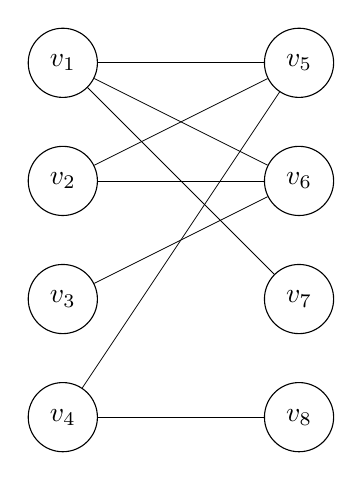
\begin{tikzpicture}
\tikzset{node style/.style={shape=circle,draw=black, inner sep=5pt,}}
                                
\node[node style] at (0, 0)     (1)     {$v_1$};
\node[node style] at (0, -1.5)   (2)     {$v_2$};
\node[node style] at (0, -3)     (3)     {$v_3$};
\node[node style] at (0, -4.5)   (4)     {$v_4$};

\node[node style] at (3, 0)     (5)     {$v_5$};
\node[node style] at (3, -1.5)   (6)     {$v_6$};
\node[node style] at (3, -3)   (7)     {$v_7$};
\node[node style] at (3, -4.5)   (8)     {$v_8$};

   
\draw[line width=0.1mm, >=latex]
            (1)     edge[right]    node {} (5)
            (1)     edge[right]    node {} (6)
            (1)     edge[right]    node {} (7)
            (2)     edge[right]    node {} (5)
            (2)     edge[right]    node {} (6)
            (3)     edge[right]    node {} (6)
            (4)     edge[right]    node {} (5)
            (4)     edge[right]    node {} (8)
;
\end{tikzpicture}
\caption{Beispiel eines bipartiten Graphen}
\label{fig:bipstd}
\end{figure}
\red{überleitung}
Für einen \ct ist vor allem der Begriff der Nachbarschaft, genauer der gemeinsamen und disjunkten 
Nachbarschaft, entscheidend.
\begin{definition}[Nachbarschaft]~\\
Ein Knoten $u \in V$ heißt \textbf{benachbart} (oder \fett{adjazent}) zu einem 
anderen Knoten $v \in V$, wenn es eine Kante $\{u,v\} \in E $ gibt. Die Menge $N(u)$ aller adjazenten Knoten
von $u$ nennt man \fett{Nachbarschaft}.
\end{definition}
\begin{definition}[gemeinsame und disjunkte Nachbarschaft]~\\
	Die \fett{gemeinsame} Nachbarschaft $N_{c}(u,v)$ zweier Knoten $u$ und $v$ ist die Menge aller Knoten, die sowohl
	zu $u$ als auch zu $v$ adjazent sind. In der \fett{disjunkten} Nachbarschaft $N_{d}(u,v)$ von $u$ und $v$ sind dagegen 
	alle Knoten die nur zu einem der beiden Knoten adjazent sind. \\
	Es gilt also $N_{c}(u,v) = N(u) \cap N(v)$ und $N_{d}(u,v) = \big(N(u) \cup N(v)\big)\setminus \big(N(u) \cap N(v) \big)$
\end{definition}
\red{Dabei bemerken wir, dass in einem Bipartiten Graphen zwei Knoten aus einer Partitionsklasse nie\dots\dots
}
\begin{definition}[Knotengrad]~\\
Der \fett{Grad} eines Knotens $v \in V$ wird mit $\deg(v)$ bezeichnet und entspricht die Anzahl
der adjazenten Knoten von $v$. Es gilt also $\deg(v) = |N(v)|$ für alle Knoten $v\in V$.

\end{definition}
\begin{definition}[Gradsequenz]~\\
Die \fett{Gradsequenz} eines Graphen $G = (V,E)$ mit $|V| = n$ Knoten ist gegeben durch das Tupel
$D = (d_{1}, \dots, d_{n})$, wobei $d_{i} = \deg(v_{1})$ der Grad des Knotens $v_{i}$ ist.
\end{definition}
\red{in abbildung ... hat man grade soundso, sequenz so}





%%%%%%%%%%%%%%%%%%%%%%%%%%%%%%%%%%%%%%%%%%%%%%%%%%%%%%%%%%%%%%%%%%%%%%%%
%%%%%% NetworKit
%%%%%%%%%%%%%%%%%%%%%%%%%%%%%%%%%%%%%%%%%%%%%%%%%%%%%%%%%%%%%%%%%%%%%%%%
\section{\nk}

\nk \cite{nk} ist ein Open-Source Projekt, dass es zum Ziel hat, ''Werkzeuge für die
Analyse großer Netzwerke, in den Größenordnungen von Tausenden bis Milliarden 
von Kanten, zur Verfügung zu stellen''.
\footnote{aus \cite{nk} abgerufen am 10.2.2020}
\\
Innerhalb von \nk Gibt es einfache Graph Datenstrukturen \red{blabla}
\\
Man kann es mit python nutzen \red{blabla}





%%%%%%%%%%%%%%%%%%%%%%%%%%%%%%%%%%%%%%%%%%%%%%%%%%%%%%%%%%%%%%%%%%%%%%%%
%%%%%% Datenstruktur
%%%%%%%%%%%%%%%%%%%%%%%%%%%%%%%%%%%%%%%%%%%%%%%%%%%%%%%%%%%%%%%%%%%%%%%%

\section{Datenstruktur}
In \nk \red{\cite{nk} muss das immer hin, wenn \nk erwähnt wird?!} werden Graphen in einer eigenen Datenstruktur gespeichert. Um den Algorithmus 
zu vereinfachen, wird der Graph in eine einfachere Datenstruktur transformiert. Dazu erstellen wir 
eine Art Adjazenzlistendarstellung des Graphen, wobei jedoch keine echten verketteten
Listen verwendet werden, sondern lediglich Vektoren. 
Es wird also für einen Knoten
$v \in V$ ein Vektor erstellt, indem alle adjazenten Knoten gespeichert sind.
Da wir ausschließlich bipartite Graphen betrachten werden, speichern wir noch in 
einem weiteren Vektor die Knoten von einer der beiden Bipartitionsklassen \red{die größere?}.
\\
Die Vektoren sind dabei vom C++ Datentyp \texttt{std::vector}.

\red{WAS muss die Datenstruktur können? -- Zwei Knoten zufällig auswählen, -- Nachbarschaften berechenen -- 
Nachbarn tauschen--}


%%%%%%%%%%%%%%%%%%%%%%%%%%%%%%%%%%%%%%%%%%%%%%%%%%%%%%%%%%%%%%%%%%%%%%%%
%%%%%% Global Curveball
%%%%%%%%%%%%%%%%%%%%%%%%%%%%%%%%%%%%%%%%%%%%%%%%%%%%%%%%%%%%%%%%%%%%%%%%

\section{Global Curveball \red{(auf bipartiten Graphen)}}
Wie \red{in der Einleitung beschrieben}, ist \gc ein Verfahren zum Randomisieren von Graphen.
Dabei ist als Eingabe ein beliebiger bipartiter Graph gegeben, der in einen \red{anderen/zufälligen}
Graph mit äquivalenter Gradsequenz transformiert werden soll.
\\
Die Aufgabe ist also, bei einer gegebenen Gradsequenz $D$, eine uniform verteilte \red{Stichprobe???}
aus der Menge aller Graphen mit Gradsequenz $D$ zurückzugeben. Durch das Ausführen von \gc 
bleibt also für jeden Knoten $v\in V$ sein Grad $\deg(v)$ erhalten. \red{(aus survey übernommen)}
\\
\\



~\\
\\
\\\
\\


\gc ist eine Variante vom ETCTS kp..

gradsequenz

MARKOV
äääöööÄÖ

%%%%% CURVEBALL TRADE auf graph
\begin{figure}[h]
\centering
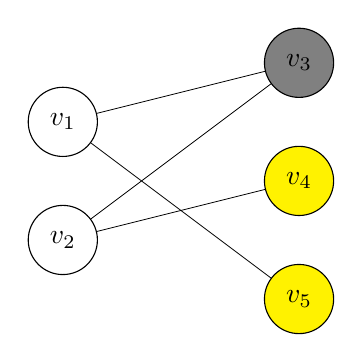
\begin{tikzpicture}
		\tikzset{node style/.style={shape=circle,draw=black, inner sep=5pt,}}
                                
\node[node style] at (0, -0.75)     (1)     {$v_1$};
\node[node style] at (0, -2.25)   (2)     {$v_2$};


\node[node style, fill=gray] at (3, 0)     (5)     {$v_3$};
\node[node style, fill=yellow] at (3, -1.5)   (6)     {$v_4$};
\node[node style, fill=yellow] at (3, -3)   (7)     {$v_5$};


   
\draw[line width=0.1mm, >=latex]
            (1)     edge[right]    node {} (5)
            (1)     edge[right]    node {} (7)
            (2)     edge[right]    node {} (5)
            (2)     edge[right]    node {} (6)

;
\end{tikzpicture}
\hspace{2cm}
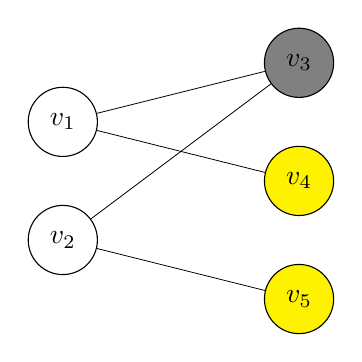
\begin{tikzpicture}
\tikzset{node style/.style={shape=circle,draw=black, inner sep=5pt,}}
                                
\node[node style] at (0, -0.75)     (1)     {$v_1$};
\node[node style] at (0, -2.25)   (2)     {$v_2$};

\node[node style, fill=gray] at (3, 0)     (5)     {$v_3$};
\node[node style, fill=yellow] at (3, -1.5)   (6)     {$v_4$};
\node[node style, fill=yellow] at (3, -3)   (7)     {$v_5$};


\draw[line width=0.1mm, >=latex]
            (1)     edge[right]    node {} (5)
            (1)     edge[right]    node {} (6)
            (2)     edge[right]    node {} (5)
            (2)     edge[right]    node {} (7)

;
\end{tikzpicture}
\caption{Beispiel eines Curveball-Tausches}
\label{fig:curveball_trade_graph}
	
\end{figure}



%%%%% CURVEBALL TRADE auf Vektor
\begin{figure}[h]
\centering
  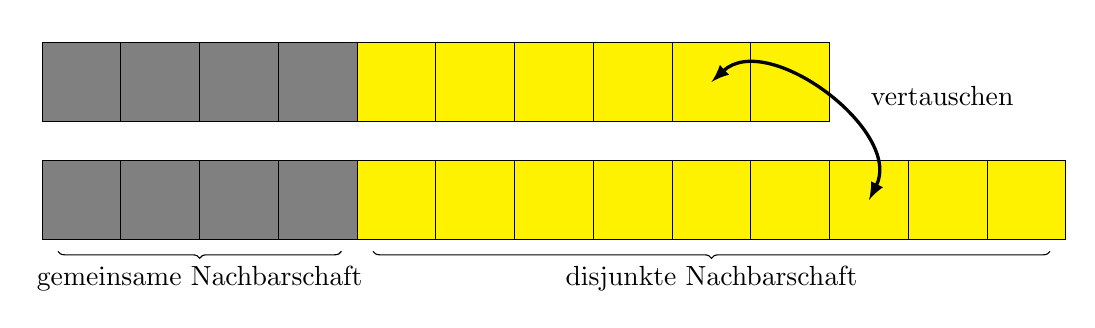
\begin{tikzpicture}[decoration=brace]
      
      
    %% COMMON FÄRBEN  
    \foreach \x in {0,1,2,3}
		{
			\fill [ fill =gray, draw =black ]  (\x ,0) rectangle (\x+1 ,1) ;
			\fill [ fill =gray, draw =black ]  (\x ,-1.5) rectangle (\x+1 ,-0.5) ;
		};

    %% DISJOINT OBEN FÄRBEN  
    \foreach \x in {4,5,6,7,8,9}
		{
			\fill [ fill =yellow, draw =black ]  (\x ,0) rectangle (\x+1 ,1) ;
		};
		
	%% DISJOINT UNTEN FÄRBEN  
    \foreach \x in {4,5,6,7,8,9,10,11,12}
		{
			\fill [ fill =yellow, draw =black ]  (\x ,-1.5) rectangle (\x+1 ,-0.5) ;
		};
    
    
    
    % untere geschweifte Klammer mit Text darunter:
    \draw[decorate, yshift=-1ex] (3.8,-1.5) -- node[below=0.4ex] {gemeinsame Nachbarschaft} (0.2,-1.5);
    \draw[decorate, yshift=-1ex] (12.8,-1.5) -- node[below=0.4ex] {disjunkte Nachbarschaft} (4.2,-1.5);


	\draw[bend left=80, <->,>=latex, very thick] (8.5,0.5) to  node[right= 3ex] {vertauschen} (10.5,-1) ;

  \end{tikzpicture}
  \caption{Beispiel für einen Curveball-Tausch}
  \label{fig:curveball_trade_vector}
  
\end{figure}




\red{Wir betrachten wie die einzelnen cb trades ausgeführt werden...}






%%%%%%%%%%%%%%%%%%%%%%%%%%%%%%%%%%%%%%%%%%%%%%%%%%%%%%%%%%%%%%%%%%%%%%%%
%%%%%% Parallelität
%%%%%%%%%%%%%%%%%%%%%%%%%%%%%%%%%%%%%%%%%%%%%%%%%%%%%%%%%%%%%%%%%%%%%%%%

\section{Parallelisierung}

\red{OPENMP UND SO...}
